\chapter{Introduction}\label{chap_Introduction}

At present, the world population has extremely increased to 8 billions of persons generating more natural resource consumption and placing extraordinary demands on agriculture and ecosystem services. As specie, we have developed amazing technology: telescopes (\href{https://webbtelescope.org/news/first-images/gallery}{Webb Space Telescope}) able to watch the universe through great solution, powerful and immense particle accelerator (\href{https://www.google.com/search?q=lhc&rlz=1C1ALOY_esCO977CO977&oq=LHC&aqs=chrome.0.0i67j46i199i465i512j0i512l8.3040j0j7&sourceid=chrome&ie=UTF-8}{LHC}) where many particles have been discovered and studied, or even extraordinarily computers that make possible to simulate an entire gene of DNA using a billion-atom bio-molecules int the \href{https://www.lanl.gov/org/ddste/aldsc/index.php}{Los Alamos National Laboratory}. Nevertheless, our natural resources demanding has reached a unsustainable point where we consume much more than we produce leading the malnourished of an important part to the whole population, more than a billion of persons. Hence, as a scientist we have to keep in mind solutions for a conserve the planet and ecosystems \cite{Foley2011}.

\begin{minipage}{0.48\linewidth}
\begin{figure}[H]
    \centering
    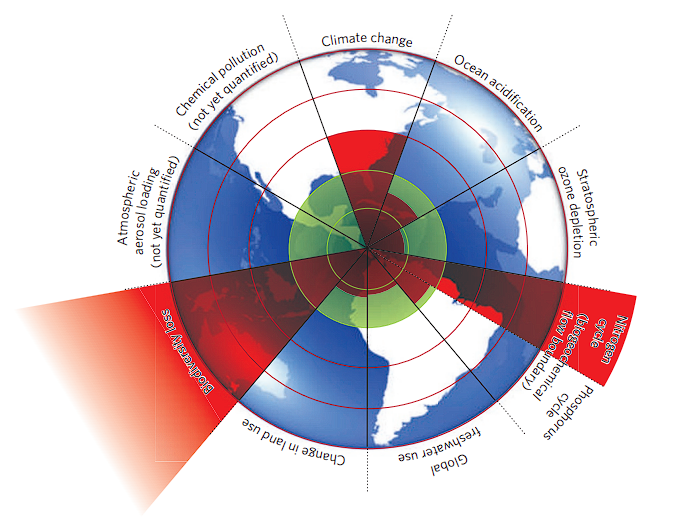
\includegraphics[width=\linewidth]{Images/biodiversity_loss.png}
    \caption{Nine planetary systems are studied in order to make a safe operating space for humanity. The green shaded region represents the safe operating system space while the red represents an estimate of the current position for each variable showing the safe values have already been exceeded.\cite{save_space}}
    \label{fig:biodiversity_loss}
\end{figure}
\end{minipage} \hfill
\begin{minipage}{0.45\linewidth}
\begin{figure}[H]
    \centering
    \includegraphics[width=\linewidth]{Images/ecosystem.png}
    \caption{Scheme of world interactions with humans and world, ecosystem functions and services for living beings. \cite{Cardinale2012}}
    \label{fig:ecosystem}
\end{figure}
\end{minipage}
\vspace{15pt}

But, how can we preserve the ecosystems? what are the boundaries that human beings must keep to avoid unacceptable environmental changes? These questions and many other have being answered with the goal to identify and quantify what are the principal systems and events that affect the most the world environment. A naive idea may be that the most important factor of environment loss is the climate change but research have shown that even if it does impact the ecosystem, it is not the main cause of the loss. Good indexes of  environmental change describing may include the biodiversity loss and  human
interference with the nitrogen cycle \ref{fig:biodiversity_loss}, furthermore they may include some food security and environmental goals to have a sustainable process.    

\begin{figure}[H]
    \centering
    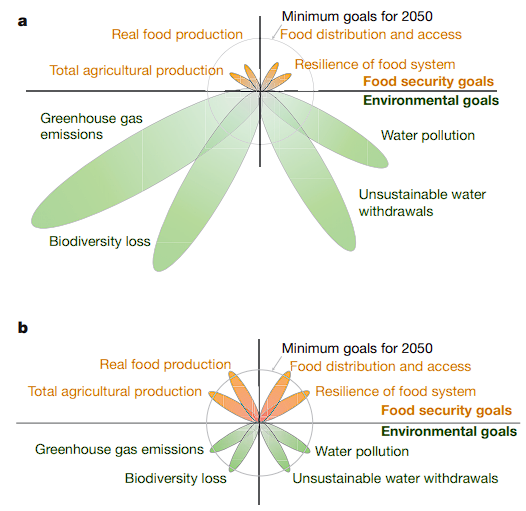
\includegraphics[width=0.8\linewidth]{Images/security.png}
    \caption{Meeting goals for food security and environmental sustainability by 2050. . Qualitatively illustration of a subset of the goals agriculture must meet in the coming decades. At the top, we outline four key food security goals: increasing total agricultural production, increasing the supply of food (recognizing that agricultural yields are not always equivalent to food), improving the distribution of and access to food, and increasing the resilience of the whole food system. At the bottom, we illustrate four key environmental goals agriculture must also meet: reducing greenhouse gas emissions from agriculture and land use, reducing biodiversity loss, phasing out unsustainable water withdrawals, and curtailing air and water pollution from agriculture. \cite{Cardinale2012}}
    \label{fig:security}
\end{figure}

Hence, the ecosystems preservation should include the birds population conservation, a good ecosystem richness index, since birds are anywhere and have an important rule for the ecosystems. Birds offers many services to society: pollination, spread seeds, decompostion, control pests, and even their pop is a fertilizer, so birds transform entire landscapes making them richer in biodiversity and if their missing will causes big impacts to the ecosystem process, as may be the case of Colombia that is ranked as the country with the largest variety of birds in the world. But this it not all, birds have also been studied to understand the human brain and learning process, and even human sound production. Birds have many similarities with humans: they learn to sing from a tutor \cite{tutor} (as humans learns to speak by hearing and repeating other humans vocalizations) and then process and reinforce this information by signing while they are sleeping\footnote{their brain sends electrical signals to the muscles, without sound generation, making a singing learning reinforcement by repeating the neurons activities while they are sleeping} \cite{brain_to_syllables, sleep} showing that even when humans learning is more complicated birds can be used to explore and test human neurology; other articles explore the analogy between birdsong syllables and music theory reveling music-like dynamic structure in songbird rhythms \cite{music_birdsongs}; among others. \\

In the process of studying similarities between birds an humans, computer scientist have used the current audio signal processing and machine learning ideas to contribute to the birds conservation problem. Those research have studied how recognize, identify, and classify birds by their birdsong or photography. Awesome research and tools have been created making possible to identity birds with just an smartphone, as does the \href{https://merlin.allaboutbirds.org/sound-id/}{Merlin Sound ID} app develop by the Cornell Lab of Ornithology. However, in spite of the huge quantity of birdsongs recorded just a few of them are individual birdsongs and have great sound quality, with low noise level and high syllables spectral resolution, which leads to a scarcity of individual birdsongs audio records. As physicist, I have been always interested in how sound is produced and how physical models and computer tools can be used to generate realistic data. In  this way, I started to study the physics of sound production and how is it simulate, mostly in music instruments, with the propose to generate synthetic sounds. Since music have been widely investigated, there are many simulations available on internet that simulate different instruments, in fact, you can find a huge quantity of sound simulations and even vocal fold simulation, human sound production.\\

This work present an study and packing of the motor gestures physical model, a python package called \href{https://github.com/saguileran/birdsongs/}{birdsongs}. \vspace{5pt}

\begin{minipage}{0.6\linewidth}
The necessary concepts and equations are describe in the literature review chapter \ref{chap_lit_review}. Next, the problem of birdsongs production and its background is explain in the chapter \ref{chap_problem_background} where at the end an automatization is proposed and discussed using optimization theory and algorithms. The programming model implementation and automatizing, solution of a minimization problem, is described and explain in the chapter \ref{chap_methodology} followed by the results and discussed, chapter \ref{chap_results}. Finally, some conclusion are present in the chapter \ref{chap_conclusions} where the package bounds and future works are specified.
\end{minipage}\hfill
\begin{minipage}{0.35\linewidth}
\begin{figure}[H]
    \centering
    
\includegraphics[width=\linewidth]{Images/bird_logo.png}
    \caption{\href{https://github.com/saguileran/birdsongs}{birdsongs}: a Python package to analyze, visualize and generate synthetic birdsongs using the\textit{ motor gestures model}. }
    \label{fig:logo}
\end{figure}
\end{minipage}